\documentclass[portrait,final,a0paper,]{baposter}

\usepackage[francais]{babel}
\usepackage[utf8]{inputenc}
\usepackage[T1]{fontenc}

\usepackage{calc}
\usepackage{graphicx}
\usepackage{amsmath}
\usepackage{amssymb}
\usepackage{relsize}
\usepackage{multirow}
\usepackage{rotating}
\usepackage{bm}
\usepackage{enumitem}
\usepackage{url}
\usepackage{booktabs}
%\usepackage{multicol}
\usepackage{xcolor}
\usetikzlibrary{calc}

\usepackage{tabularx}


%\usepackage{times}
\usepackage{helvet}
%\usepackage{bookman}
%\usepackage{palatino}
\renewcommand*{\familydefault}{\sfdefault}

\newcommand{\captionfont}{\footnotesize}

\graphicspath{{images/}}

\setlength{\columnsep}{1.5em}
\setlength{\columnseprule}{0mm}

\newcommand{\marktikz}[1]{ \tikz[remember picture,overlay]\node (#1) {};}

%%%%%%%%%%%%%%%%%%%%%%%%%%%%%%%%%%%%%%%%%%%%%%%%%%%%%%%%%%%%%%%%%%%%%%%%%%%%%%%%
% Save space in lists. Use this after the opening of the list
%%%%%%%%%%%%%%%%%%%%%%%%%%%%%%%%%%%%%%%%%%%%%%%%%%%%%%%%%%%%%%%%%%%%%%%%%%%%%%%%
\newcommand{\compresslist}{%
\setlength{\itemsep}{1pt}%
\setlength{\parskip}{0pt}%
\setlength{\parsep}{0pt}%
}



\newcommand{\diag}[1]{\lceil#1\rfloor}
\newcommand*\circled[1]{\tikz[baseline=(char.base)]{
            \node[shape=circle,draw,inner sep=2pt,color=main,fill=main!10, line width=1pt] (char) {#1};}}

%%%%%%%%%%%%%%%%%%%%%%%%%%%%%%%%%%%%%%%%%%%%%%%%%%%%%%%%%%%%%%%%%%%%%%%%%%%%%%
%%% Begin of Document
%%%%%%%%%%%%%%%%%%%%%%%%%%%%%%%%%%%%%%%%%%%%%%%%%%%%%%%%%%%%%%%%%%%%%%%%%%%%%%

\begin{document}

%%%%%%%%%%%%%%%%%%%%%%%%%%%%%%%%%%%%%%%%%%%%%%%%%%%%%%%%%%%%%%%%%%%%%%%%%%%%%%
%%% Here starts the poster
%%%---------------------------------------------------------------------------
%%% Format it to your taste with the options
%%%%%%%%%%%%%%%%%%%%%%%%%%%%%%%%%%%%%%%%%%%%%%%%%%%%%%%%%%%%%%%%%%%%%%%%%%%%%%
% Define some colors


\definecolor{green}{rgb}{0.32,0.67,0.39}
%\definecolor{main}{rgb}{0 0.627 0.588} %canard
\definecolor{main}{rgb}{0 0.439  0.753} %bleu %0 112 192

%\hyphenation{resolution occlusions}
%%
\begin{poster}%
  % Poster Options
  {
  % Show grid to help with alignment
  grid=false,
  % Column
  columns=6,
  colspacing=1em,
  % Color style
  background=plain,%%shadetb,
  bgColorOne=gray!12,%lightestgreen!80,
  bgColorTwo=white,
  borderColor=white,%darkgreen,
  headerColorOne=white,%darkgreen,
  %headerColorTwo=lightgreen,
  headerFontColor=main,%white,
  boxColorOne=white,%lightestgreen,
  %boxColorTwo=lightgreen,
  % Format of textbox
  textborder=roundedleft,%faded,
  % Format of text header
  eyecatcher=false,
  headerborder=closed,
  headerheight=0.08\textheight,
  %textfont=\sc,% An example of changing the text font
  headershape=roundedright,
  headershade=plain,%shadelr,
  headerfont=\Large\bfseries,%\textsc, %Sans Serif
  textfont={\setlength{\parindent}{1.5em}},
  boxshade=plain,
  linewidth=2pt
  }
  % Eye Catcher
  {  }
  % Title
 {
%\begin{tikzpicture}[overlay, remember picture, inner sep=0pt, outer sep=0pt]
%  %\fill [white] ([yshift=-3cm]current page.north west) rectangle (current page.north east);
%\end{tikzpicture}
%\begin{minipage}{\linewidth}
%	\vspace{0.5cm}
%	\includegraphics[height=1cm]{logo/LABEX_CELYA.jpg} \hfill \includegraphics[height=1cm]{logo/logo_lmfa.pdf} \hfill \includegraphics[height=1cm]{logo/LVA_compact_couleur_transparent.png} \hfill   \includegraphics[trim={0 3cm 0 3cm},clip=true,height=1cm]{logo/logo_ADAPT.png}\\
%\end{minipage} 
\vspace{0.4cm}\textcolor{main}{\textbf{Débruitage de la matrice interspectrale pour l'étude des sources aéroacoustiques}}}
  % Authors
  { ~\\A. Dinsenmeyer\textsuperscript{1,2}, Q. Leclère\textsuperscript{1}, J. Antoni\textsuperscript{1}, E. Julliard\textsuperscript{3}}
  % University logo
  {  }
  
 
%%%%%%%%%%%%%%%%%%%%%%%%%%%%%%%%%%%%%%%%%%%%%%%%%%%%%%%%%%%%%%%%%%%%%%%%%%%%%%
%%% Now define the boxes that make up the poster
%%%---------------------------------------------------------------------------
%%% Each box has a name and can be placed absolutely or relatively.
%%% The only inconvenience is that you can only specify a relative position 
%%% towards an already declared box. So if you have a box attached to the 
%%% bottom, one to the top and a third one which should be in between, you 
%%% have to specify the top and bottom boxes before you specify the middle 
%%% box.
%%%%%%%%%%%%%%%%%%%%%%%%%%%%%%%%%%%%%%%%%%%%%%%%%%%%%%%%%%%%%%%%%%%%%%%%%%%%%%
 
 \headerbox{Contexte}{name=contexte,column=0,span=4}{
Verrous scientifiques et technologiques

Débriutage expé\\
mise à zéro ou soustraction : pourquoi ?\\
définition CSM\\~\\~\\~\\~\\
 }
 

 
 \headerbox{Méthode proposée}{name=methode,below=contexte,below=contexte,column=0,span=6}{
 
 \noindent\begin{minipage}[t]{0.24\textwidth}
	\centering
	\resizebox{0.5cm}{!}{\circled{\textbf{1}}} \marktikz{step1out}  \\[1ex]
	 {\bfseries Choisir un modèle statistique}\\
	 $\displaystyle \bm{M\left( \bm{\theta} \right)}$\\[1em]
 
	%$\displaystyle \bm{p}_j=\bm{L \diag{\alpha} c}_j+\bm{n}_j$\\
	%$\displaystyle j=1,\dots,Ns$\\[1ex]
	 	 \newlength{\larg}	\setlength{\larg}{0.3cm}	
	 	\newlength{\haut}	\setlength{\haut}{1.5cm}
	 	\setlength{\tabcolsep}{0.7ex}
	\noindent \begin{tabular}{m{1.2ex} m{0.5ex} m{2\larg+\haut+1ex} m{0.1ex}  m{\haut}}
	$\bm{S}_{pp}$ & $=$ & \centering$\bm{L \diag{\alpha} S}_{cc} \bm{\diag{\alpha} L}'$&  $+$ &  \parbox{\linewidth}{ \centering $\diag{\bm{\sigma}^2_n}$} \\[1ex]
	 & $=$  & \tikz{
	 	\node at (-2cm,0) (a) {};
	 	\draw [rectangle,main,line width=1pt,fill=main!10] (a)  rectangle  ++ (\larg,-\haut)  ; 	 
	 	\draw[rectangle,main,line width=1pt,fill=main!10] (a)++(\larg+0.1cm,-0.5\haut+0.5\larg) rectangle ++(\larg,-\larg);
		\draw[main,rectangle,line width=1pt,fill=main!10] (a)++(2\larg+0.2cm,-0.5\haut+0.5\larg) rectangle ++(\haut,-\larg);
		}
		 & $+$ 
		 &\tikz{
		\draw[main,line width=1pt]  (-1cm,0) rectangle ++(\haut,-\haut); 
		\draw[line width=1pt,main] (-1cm,0) to ++(\haut,-\haut);
		}\\
		& &
%		\tikz{
%		\node [] at (0.25cm,0cm) {\small $(M\!\!\times\!\!K$)};
%		\node [] at (0.85cm,0cm) {\small $(K\!\!\times\!\!K$)};
%		\node [] at (0.85cm,0cm) {\small $(K\!\!\times\!\!M$)};
%		}
	 \parbox{\linewidth}{ \centering \footnotesize  $(M\!\!\times\!\!K)(K\!\!\times\!\!K)(K\!\!\times\!\!M)$}
		& & \parbox{\linewidth}{ \centering \footnotesize $(M\!\!\times\!\! M)$}\\
		 & &  \parbox{\linewidth}{ $\underbrace{\hspace{\linewidth}}$\\ \centering \scriptsize Matrice à rang réduit} & & \parbox{\linewidth}{$\underbrace{\hspace{\linewidth}}$\\ \centering \scriptsize Bruit décorrélé}
	\end{tabular}	
	%Justifier le modèle : sélection d'ordre, longueur corr
	
\end{minipage}
	\hfill
\begin{minipage}[t]{0.24\textwidth}
	\centering
	\marktikz{step2in} 
	\resizebox{0.5cm}{!}{\circled{\textbf{2}}}
	\marktikz{step2out} \\[1ex]
	{ \bfseries Choix des distributions \textit{a priori}}\\[1em]
	\vspace{1em}	
	\includegraphics[width=0.9\textwidth]{modele.png}

%	\begin{align*}
%		\bm{L} &\sim \mathcal{N}_{\mathbb{C}} \left( 0,\frac{\bm{I}}{\kappa} \right)\\		
%		\bm{\alpha}& \sim \mathcal{E}(\bm{a}_{\alpha}), \label{eq:alpha} \\
%		\bm{c} &\sim  \mathcal{N}_{\mathbb{C}} ( 0 , \bm{\gamma}^2 )	\\
%		\bm{n}& \sim \mathcal{N}_{\mathbb{C}} \left( 0 , \diag{\bm{\sigma}_n^2} \right)		
%	\end{align*}
%	
%		Hyperpriors :
%	\begin{align*}
%		\bm{\gamma}^2 & \sim \mathcal{IG}( \bm{a}_{\gamma}, \bm{b}_{\gamma}) \\
%		\bm{\sigma}_n^2  & \sim \mathcal{IG} (\bm{a}_{\sigma} , \bm{b}_{\sigma})
%	\end{align*}		
\end{minipage}\hfill
\begin{minipage}[t]{0.24\textwidth}
		\centering
		{  \marktikz{step3in}\resizebox{0.5cm}{!}{\circled{\textbf{3}}}  \marktikz{step3out}  } \\[1ex]
		{\bfseries Trouver le maximum de la distribution \textit{a posteriori}}\\
		\textit{Estimer les paramètres qui expliquent au mieux les mesures}\\
		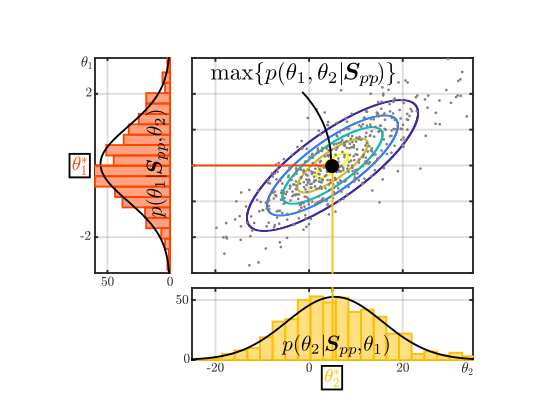
\includegraphics[width=0.9\textwidth]{gibbs.png}	
\end{minipage}
\hfill
 \begin{minipage}[t]{0.24\textwidth}
		\centering
		\marktikz{step4in}   \resizebox{0.5cm}{!}{\circled{\textbf{4}}} \marktikz{step4out} \\[1ex]
		{\bfseries Reconstruire la CSM débruitée}\\[1em]
		\includegraphics[width=0.4\textwidth]{signal.png}  \raisebox{0.15\textwidth}{\large $+$} 
\includegraphics[width=0.4\textwidth]{bruit.png}
\end{minipage}

\tikz[remember picture,overlay]{
	\draw[->,line width=1pt, main,>=latex] ($ (step1out.east)+(0,1ex)$) to [out=20,in=160] ( $ (step2in.west) + (0,1ex) $ );%
	\draw[->,line width=1pt, main,>=latex] ($ (step2out.east)+(0	,1ex)$) to [out=20,in=160] ( $ (step3in.west) + (0,1ex) $ );%
	\draw[->,line width=1pt, main,>=latex] ($ (step3out.east)+(0,1ex)$) to [out=20,in=160] ( $ (step4in.west) + (0,1ex) $ );%	
}
 }
 
   \headerbox{}{name=image,span=2,column=4,boxColorOne=gray!12,borderColor=gray!12}{
%  \begin{minipage}[t][1cm][t]{\linewidth}
% 	\centering 	
% 	\noindent \hspace{-3cm}\vspace{2cm}\includegraphics[width=12cm]{contexte.png} 
%\end{minipage}
\begin{minipage}[t][1cm][t]{\textwidth}
	\centering
	\node[inner sep=0pt,overlay,anchor=north west] () at (-1cm,1cm)  {\includegraphics[width=0.31\paperwidth]{contexte.png} };
\end{minipage}

 }
 
 
 \headerbox{Application à l'imagerie}{name=imagerie,column=0,span=6,below=methode}{
 \centering
 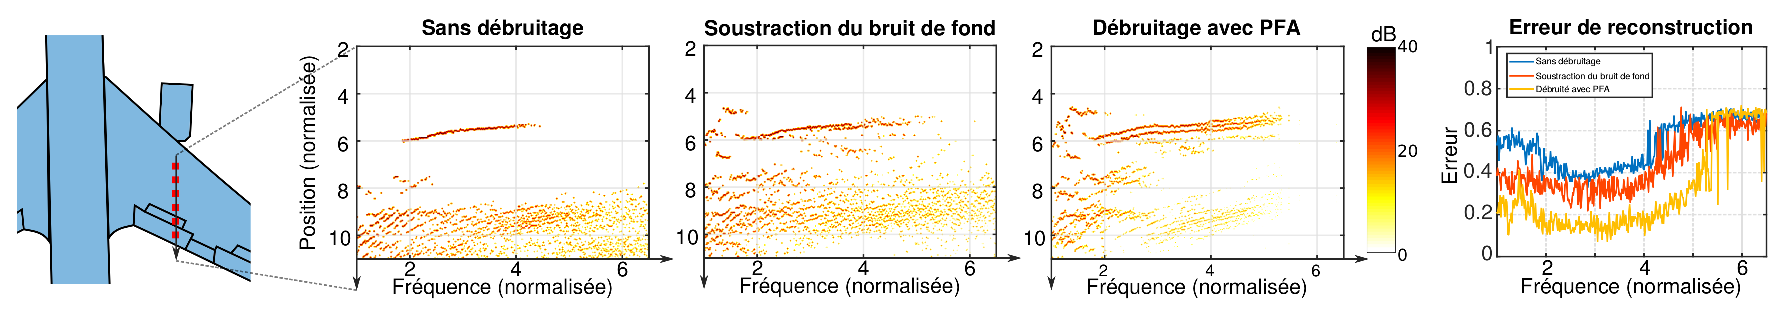
\includegraphics[width=0.9\textwidth]{imagerie_final.eps}

 
 }
 
 \headerbox{Analyse}{name=analyse,column=0, span,below=imagerie}{
 
 }
 
 \headerbox{Perspectives}{name=perspective,column=2, span=3,below=imagerie}{
 
 }
 

 \headerbox{}{name=about,column=0,span=6,below=perspective}{
  	\centering
  	 \small
	  Contact : \url{alice.dinsenmeyer@insa-lyon.fr}\\
	  \textsuperscript{1}Laboratoire Vibrations Acoustique, Villeurbanne ; 
	\textsuperscript{2}Laboratoire de Mécanique des Fluides et Acoustique, Écully ; 
	\textsuperscript{3}Airbus, Toulouse\\
 	 \includegraphics[width=3cm]{logo/LABEX_CELYA.jpg} \hfill
 	  \includegraphics[trim={0 3cm 0 3cm},clip=true,width=3cm]{logo/logo_ADAPT.png} \hfill
 \includegraphics[width=2.5cm]{logo/LVA_compact_couleur.jpg} \hfill
 \includegraphics[width=2.5cm]{logo/logo_lmfa.pdf} \hfill  
}

\end{poster}

\end{document}
